\documentclass[utf8x, xcolor=dvipsnames]{beamer}

%----------------------------------------------------------------------------------------
%	PACKAGES AND THEMES
%----------------------------------------------------------------------------------------

% Custom Theme
\usetheme{Template}

% Packages
\usepackage[ngerman]{babel}
\usepackage{lmodern}
\usepackage[T1]{fontenc}
\usepackage{inputenc}
%\usepackage[utf8]{inputenc}
\usepackage{graphicx}
\usepackage{amssymb,amsfonts,amsmath}
%\usepackage[squaren,textstyle]{SIunits}
\usepackage{siunitx}
\usepackage{hyperref}
\usepackage{textcomp}
\usepackage{booktabs}
\usepackage{xcolor,cancel}
\usepackage{multirow}
\usepackage{pifont}

\newcommand{\cmark}{\ding{51}}%
\newcommand{\xmark}{\ding{55}}%

\newcommand\hcancel[2][black]{\setbox0=\hbox{$#2$}%
\rlap{\raisebox{.45\ht0}{\textcolor{#1}{\rule{\wd0}{1pt}}}}#2}

\setbeamercovered{invisible}

\AtBeginSection[]{
  \begin{frame}
  \vfill
  \centering
  \begin{beamercolorbox}[sep=8pt,center,shadow=true,rounded=true]{title}
    \usebeamerfont{title}\insertsection\par%
  \end{beamercolorbox}
  \vfill
  \end{frame}
}

%\AtBeginSubsection[]{
%  \begin{frame}
%  \vfill
%  \centering
%  \begin{beamercolorbox}[sep=8pt,center,shadow=true,rounded=true]{title}
%    \usebeamerfont{title}\insertsubsection\par%
%  \end{beamercolorbox}
%  \vfill
%  \end{frame}
%}

%----------------------------------------------------------------------------------------
%	TITLE PAGE
%----------------------------------------------------------------------------------------

\title[PV Modulfehler]{Erkennung von Modulfehlern in Photovoltaikanlagen} % The short title appears at the bottom of every slide, the full title is only on the title page
%\subtitle{}

\author{Dominik Löwen, Tristan Nentwig, Jonas Posselt, Niklas Rettinger, Marius Warning} % Your name
\institute[FH Bielefeld] % Your institution as it will appear on the bottom of every slide, may be shorthand to save space
{
Fachhochschule Bielefeld \\ % Your institution for the title page
}
\date{23. Juni 2021} % Date, can be changed to a custom date


\begin{document}

\begin{frame}
\titlepage % Print the title page as the first slide
\end{frame}

\begin{frame}
\frametitle{Inhalt} % Table of contents slide, comment this block out to remove it
\setcounter{tocdepth}{1}
\tableofcontents % Throughout your presentation, if you choose to use \section{} and \subsection{} commands, these will automatically be printed on this slide as an overview of your presentation
\end{frame}

%----------------------------------------------------------------------------------------
%	PRESENTATION SLIDES
%----------------------------------------------------------------------------------------

%\begin{frame}
%\frametitle{}
%\end{frame}

%\begin{frame}
%\frametitle{}
%\begin{figure}
%	\includegraphics[width=\linewidth]{img/}
%\end{figure}
%\end{frame}

%\begin{frame}
%\frametitle{}
%\begin{columns}[c] % The "c" option specifies centered vertical alignment while the "t" option is used for top vertical alignment
%\column{.5\textwidth} % Left column and width
%\column{.5\textwidth} % Right column and width
%\end{columns}
%\end{frame}


%• Projektbeschreibung, interdisziplinäre Grundlagen
%• Vorstellung der Gruppenmitglieder und Ihre Rollen und Aufgaben im Team
%• KI-Fragestellungen im Projektkontext
%• SW-Realisierungen
%• Realisierung der intelligenten Datenanalyse mit Angabe von Formeln für Featurevektoren, Normalisierung und Klassifikation
%• Experimente laut wissenschaftlicher Fragestellungen, Angabe der Lern-und Testdatensätze und formale Beschreibung der konkreten Algorithmen
%• Ergebnisse laut wissenschaftlicher Fragestellungen mit Güte der Erkennungsraten
%• Demonstration der Projekt-SW
%• Fazit

%------------------------------------------------
\section[Projekt]{Projektbeschreibung}
%------------------------------------------------
\subsection{Problembeschreibung}

\begin{frame}
\frametitle{Problembeschreibung}
\begin{itemize}
	\item Stringdaten aus dem Forschungsprojekt PVDigital 4.0 werden gesammelt und analysiert
	\item Anomalien können in den Daten auftreten
	\item Anomalien sollen analysiert werden, um Fehlerfälle zu erkennen
	\item Fehlerfälle können z.B. defekte Dioden sein
	\item Für die Analyse werden Methoden des Maschine Learnings verwendet
\end{itemize}
\end{frame}

\subsection{Projektteam}

\begin{frame}
\frametitle{Projektteam}
\begin{itemize}
	\item Jonas Posselt: Team Leiter, Datenaufbereitung, Mathematik
	\item Niklas Rettinger: Repoverwaltung, Datenvisualisierung
	\item Tristan Nentwig: Datenvisualisierung, Machine Learning
	\item Marius Warning: Datenaufbereitung, Dokumentation
	\item Dominik Löwen: Datenaufbereitung, Dokumentation
\end{itemize}
\end{frame}

%------------------------------------------------
\section[Grundlagen]{Interdisziplinäre Grundlagen}
%------------------------------------------------
\subsection{Photovoltaik}

\begin{frame}
\frametitle{Photovoltaik Technische Grundlagen}
\begin{itemize}
	\item Basieren auf Halbleitern, die nur bei richtigen Bedingungen leitend sind
	\item Stromerzeugung basiert auf zwei Prozessen
	\begin{itemize}
		\item \textbf{Innere Photoeffekt}\\
			  Tritt innerhalb der Halbleiter auf. Durch Photonen entstehen Elektron-Loch-Paare und ermöglicht elektrischen Stromfluss
		\item \textbf{Äußere Photoeffekt}\\
		 	  Herauslösen von Eleketronen aus einer Halbleiter- oder Matalloberfläche durch Bestrahlung
	\end{itemize}
\end{itemize}
\end{frame}

\begin{frame}
\frametitle{Photovoltaik-Modularten}
Arten unterscheiden sich durch den Zelltypen. Die PV-Module mit verschiedenen Zelltypen haben einen unterschiedlichen Wirkungsgrad. 
\begin{figure}
	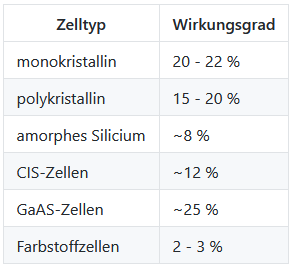
\includegraphics[scale=0.7]{images/PV_Modultypen_unterschiede.PNG}
\end{figure}
\end{frame}

\subsection{Modulfehler}

\begin{frame}
\frametitle{Modulfehler}
Zellen mit Fehlern erzeugen proportional zur betroffenen Fläche weniger Strom. Je nach größe des Bereichs kann ein ganzer Modulstring abgeschaltet werden\\
Fehlerarten: 
\begin{itemize}
	\item Konstante Fehler\\
		  Verschmutzung, Verschattung und Degradierung
	\item Sporadische Fehler\\
		  Stromausfall, Glasbruch, Zellbruch, Kurzschluss an Dioden, Schnee, Fehlerhafte Isolierung
	\item Folgefehler \\
		  Hotspots
\end{itemize}
\end{frame}

\subsection{Deep Learning}

\begin{frame}
\frametitle{Perzeptron}
\begin{itemize}
	\item Erweitertes Modell eines künstlichen Neurons
	\item Signale müssen nicht mehr binär sein
	\item Eingangssignale sind gewichtet
	\item Eingangssignale werden in einer Aktivierungsfunktion verwendet
\end{itemize}
\begin{figure}
	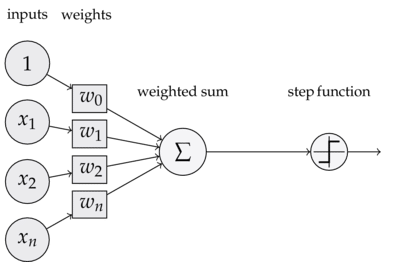
\includegraphics[scale=0.5]{images/perceptron.png}
\end{figure}
\end{frame}

\begin{frame}
\frametitle{Deep Learning}
\begin{itemize}
	\item Deep Learning gehört zum Machine Learning und beschreibt ein Neuronales Netz, das mind. 3 Ebenen hat
	\item Versucht das Menschliche Gehirn nachzuahmen
	\item Kann in Unüberwachtes- und Überwachtes Lernen eingeteilt werden
\end{itemize}
\end{frame}

\begin{frame}
\frametitle{Rekurrente neuronale Netze}
\begin{itemize}
	\item Rückwärts gerichtete Verbindungen innerhalb des Netzes
	\item Ermöglicht verarbeitung Zeitlicher Muster
	\item Neuronen erhalten zusätlich zu Eingabedaten die vorherigen Eingabedaten
	\item Nachteil: Eingabedaten von frühen Zeiten verblassen, durch ständige Transformation
	\item LSTM-Zellen besitzen zwei Zustandsvektoren, um kurzfristige und langfristige Merkmale zu speichern
\end{itemize}
\end{frame}

\begin{frame}
\frametitle{Support-Vector-Machine}
\begin{itemize}
	\item Algorithmus für die Klassifizierung von Daten mithilfe von Überwachtem Lernen
	\item Hyperplanes werden verwendet um verschiedene Daten voneinader zu unterscheiden
\end{itemize}
\begin{figure}
	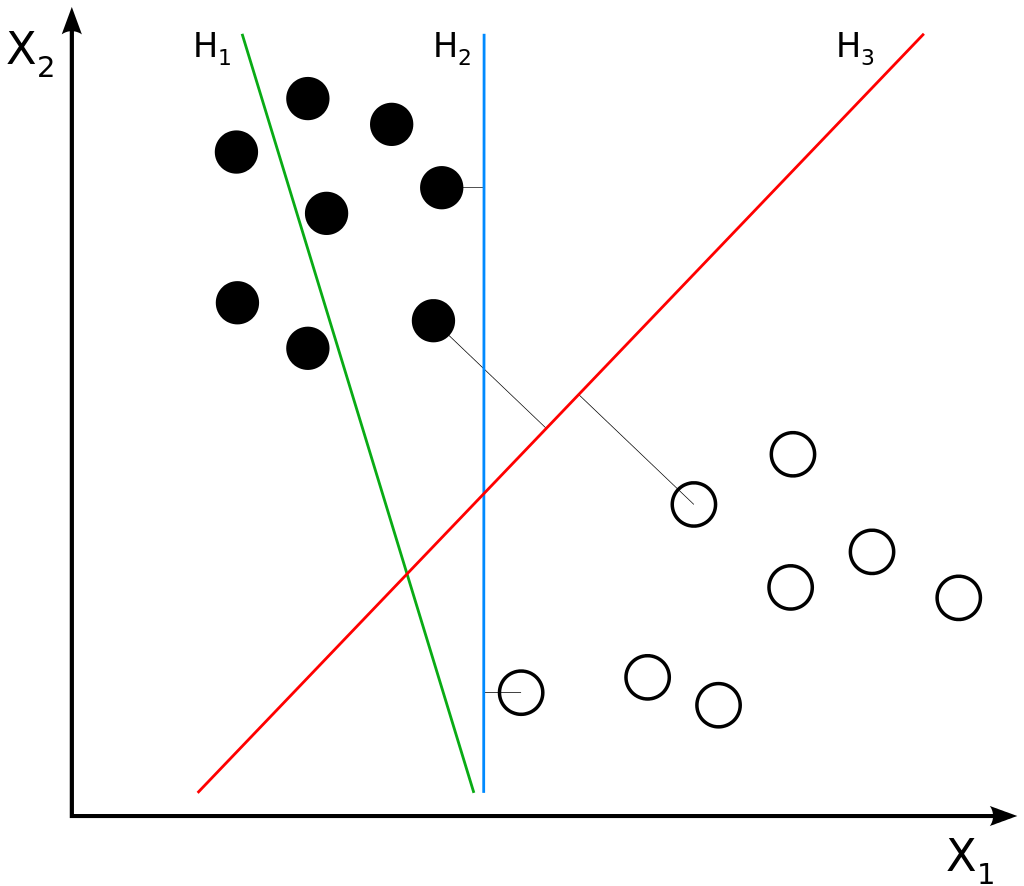
\includegraphics[scale=0.15]{images/Svm_separating_hyperplanes.png}
\end{figure}
\end{frame}

%------------------------------------------------
\section[Fragestellungen]{KI-Fragestellungen}
%------------------------------------------------

\begin{frame}
\frametitle{Forschungsfragen}
\begin{enumerate}
	\item Lassen sich Modulfehler von Photovoltaikanlagen mit Hilfe von maschinellem Lernen anhand von Leistungs- und Wetterdaten zuverlässig erkennen und klassifizieren?\newline
	\item Lässt sich die Erkennung von Modulfehlern durch das Einbeziehen simulierter Daten verbessern?
\end{enumerate}
\end{frame}

%------------------------------------------------
\section[Realisierungen]{Software-Realisierungen}
%------------------------------------------------

\begin{frame}
\frametitle{Verwendete Bibliotheken}
\begin{figure}
	
\includegraphics[width=5cm,clip]{images/pandas.jpg}
	
\includegraphics[width=3cm,clip]{images/seaborn.png}
\end{figure}
\begin{figure}
	
\includegraphics[width=4cm,clip]{images/sklearn.png}
	
\includegraphics[width=4cm,clip]{images/tensorflow.png}
\end{figure}
\end{frame}


\begin{frame}
\frametitle{Code-Struktur}
\begin{figure}
	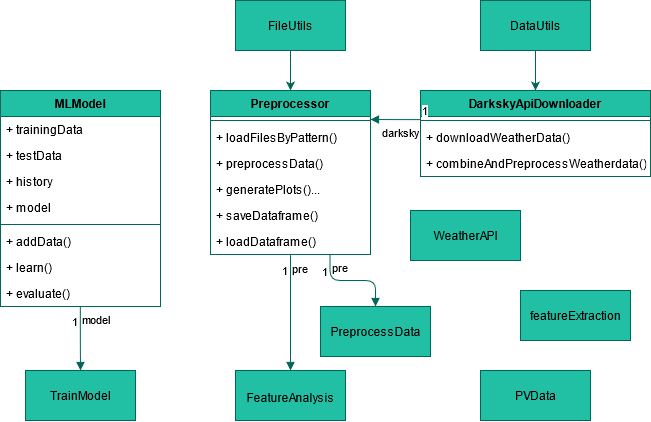
\includegraphics[width=\textwidth,clip]{images/KlassenStruktur.png}
\end{figure}
\end{frame}

%------------------------------------------------
\section{Datenanalyse}
%------------------------------------------------
\subsection{Datenbasis}

\begin{frame}
\frametitle{Datenbasis}
\begin{itemize}
	\item PV Daten (real)
	\begin{itemize}
		\item verschiedene Anlagen (Standort, Ausrichtung)
		\item geparst und auf Zellebene umgerechnet
		\item 15 Min. Intervall
		\item teilweise bekannte Fehler\newline
	\end{itemize}
	\item PV Daten (simuliert)
	\begin{itemize}
		\item Schatten- und Diodenfehler
		\item 5 Min. Intervall\newline
	\end{itemize}
	\item Wetterdaten
	\begin{itemize}
		\item Darksky API
		\item stündlich
	\end{itemize}
\end{itemize}
\end{frame}

\begin{frame}
\frametitle{Datenaufbereitung}
\begin{itemize}
	\item Säubern:
	\begin{itemize}
		\item NaN Wert am Tagesanfang/ende
		\item nicht benötigte Spalten\newline
	\end{itemize}
	\item Transformation: Zeitstempel im Datetime-Format\newline
	\item Konsolidierung:
	\begin{itemize}
		\item PV-Daten $\rightarrow$ Standortkoord. + Zeitstempel $\rightarrow$ Wetterdaten
		\item Resampling Wetterdaten auf 15 Min. Intervall
		\item Verbindung anhand Zeitstempel\newline
	\end{itemize}
	\item Normierung: Hyperwürfel

\end{itemize}
\end{frame}

\subsection{Featurevektoren}

\begin{frame}
\frametitle{Features}
\begin{columns}[t]
	\column{.5\textwidth}
	PV-Anlage:
	\begin{itemize}
		\item Edaily
		\item AcPower
		\item Dcp
		\item Dci
		\item Dcu
	\end{itemize}
	\column{.5\textwidth}
	Wetter:
	\begin{itemize}
		\item temperature
		\item pressure
		\item dewPoint
		\item cloudCover
		\item visibility
		\item uvIndex
		\item humidity
		\item ...
	\end{itemize}
\end{columns}
\end{frame}

\begin{frame}
\frametitle{Wetterdaten}
\begin{figure}
	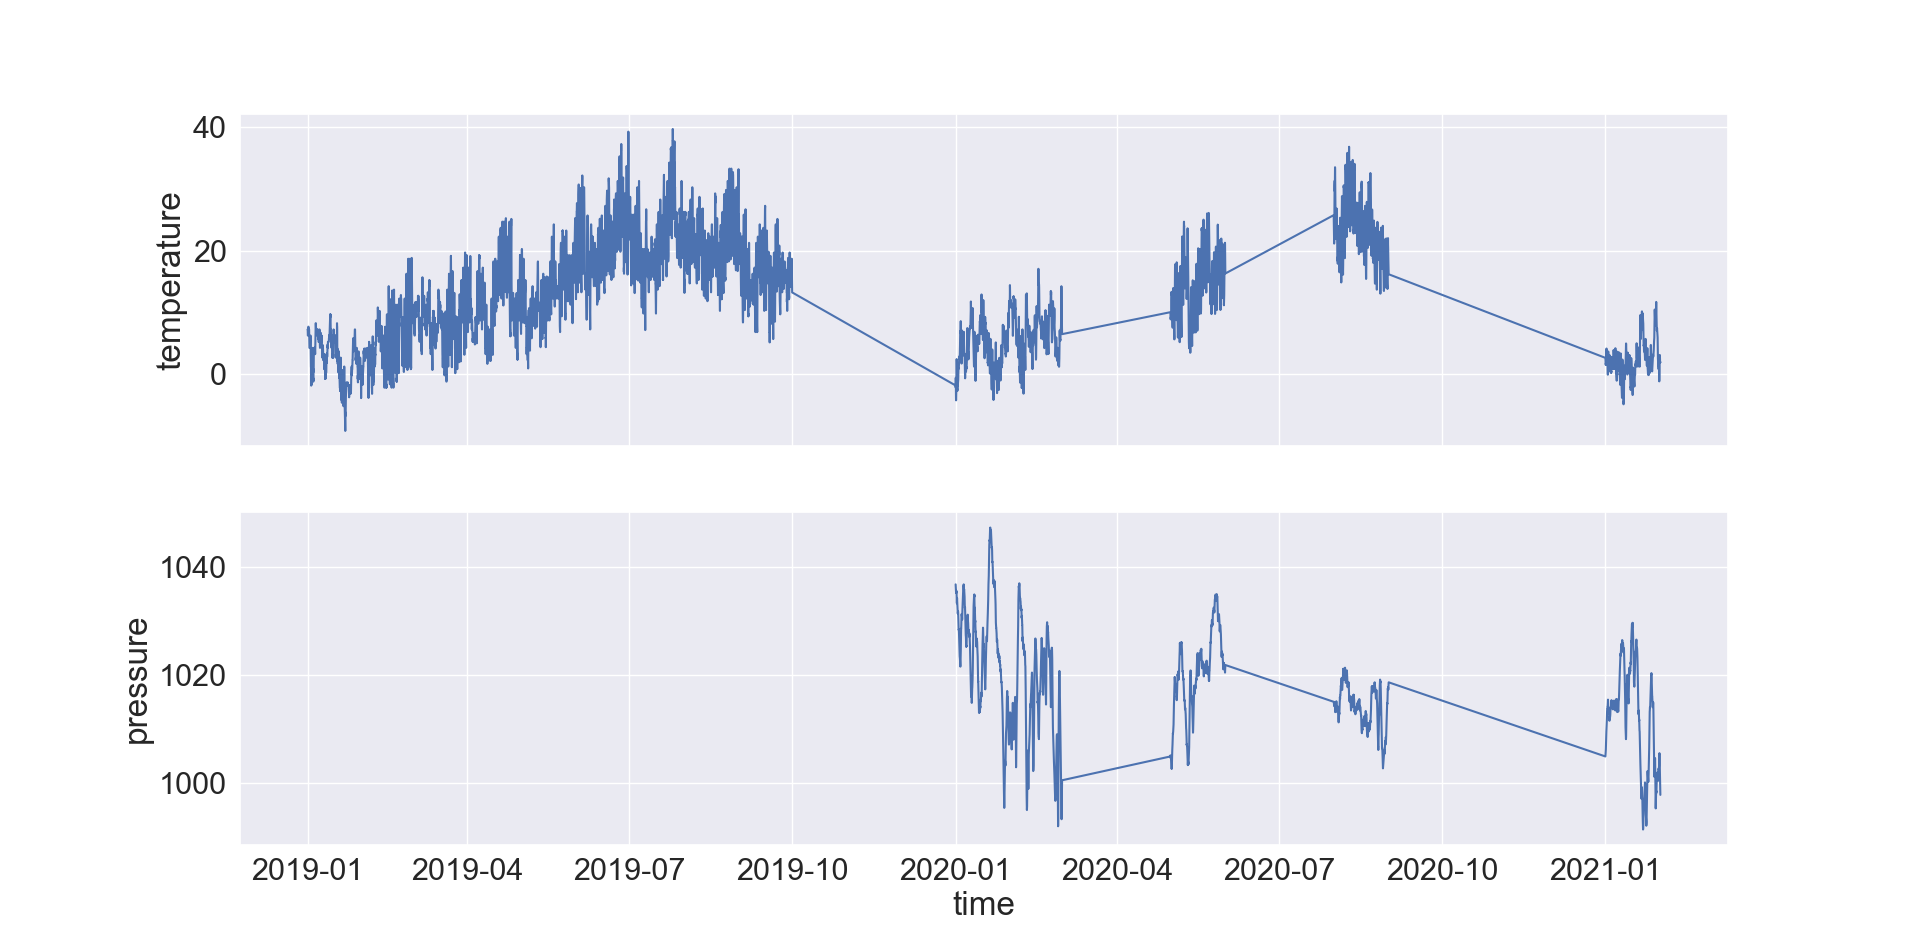
\includegraphics[width=\textwidth,trim={3cm 0.5cm 3cm 2.5cm},clip]{images/Weather1.png}
\end{figure}
\end{frame}

\begin{frame}
\frametitle{Wetterdaten}
\begin{columns}[c]
	\column{.5\textwidth}
		Visibility:
		\begin{itemize}
			\item Häufung bei 10 und 16\newline
			\item Mischung verschiedener Einheiten (Meilen + Kilometer)
		\end{itemize}
	\column{.5\textwidth}
		\begin{figure}
			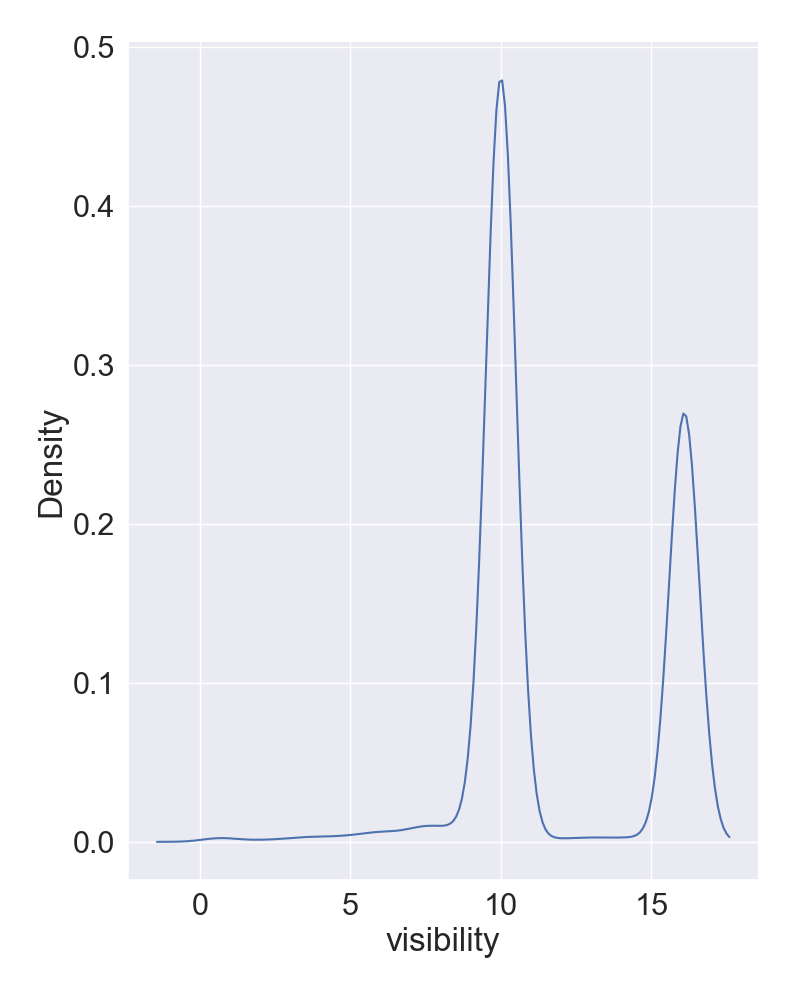
\includegraphics[width=\textwidth]{images/visibility.png}
		\end{figure}
\end{columns}
\end{frame}

\begin{frame}
\frametitle{Korrelation (Heatmap)}
\begin{figure}
	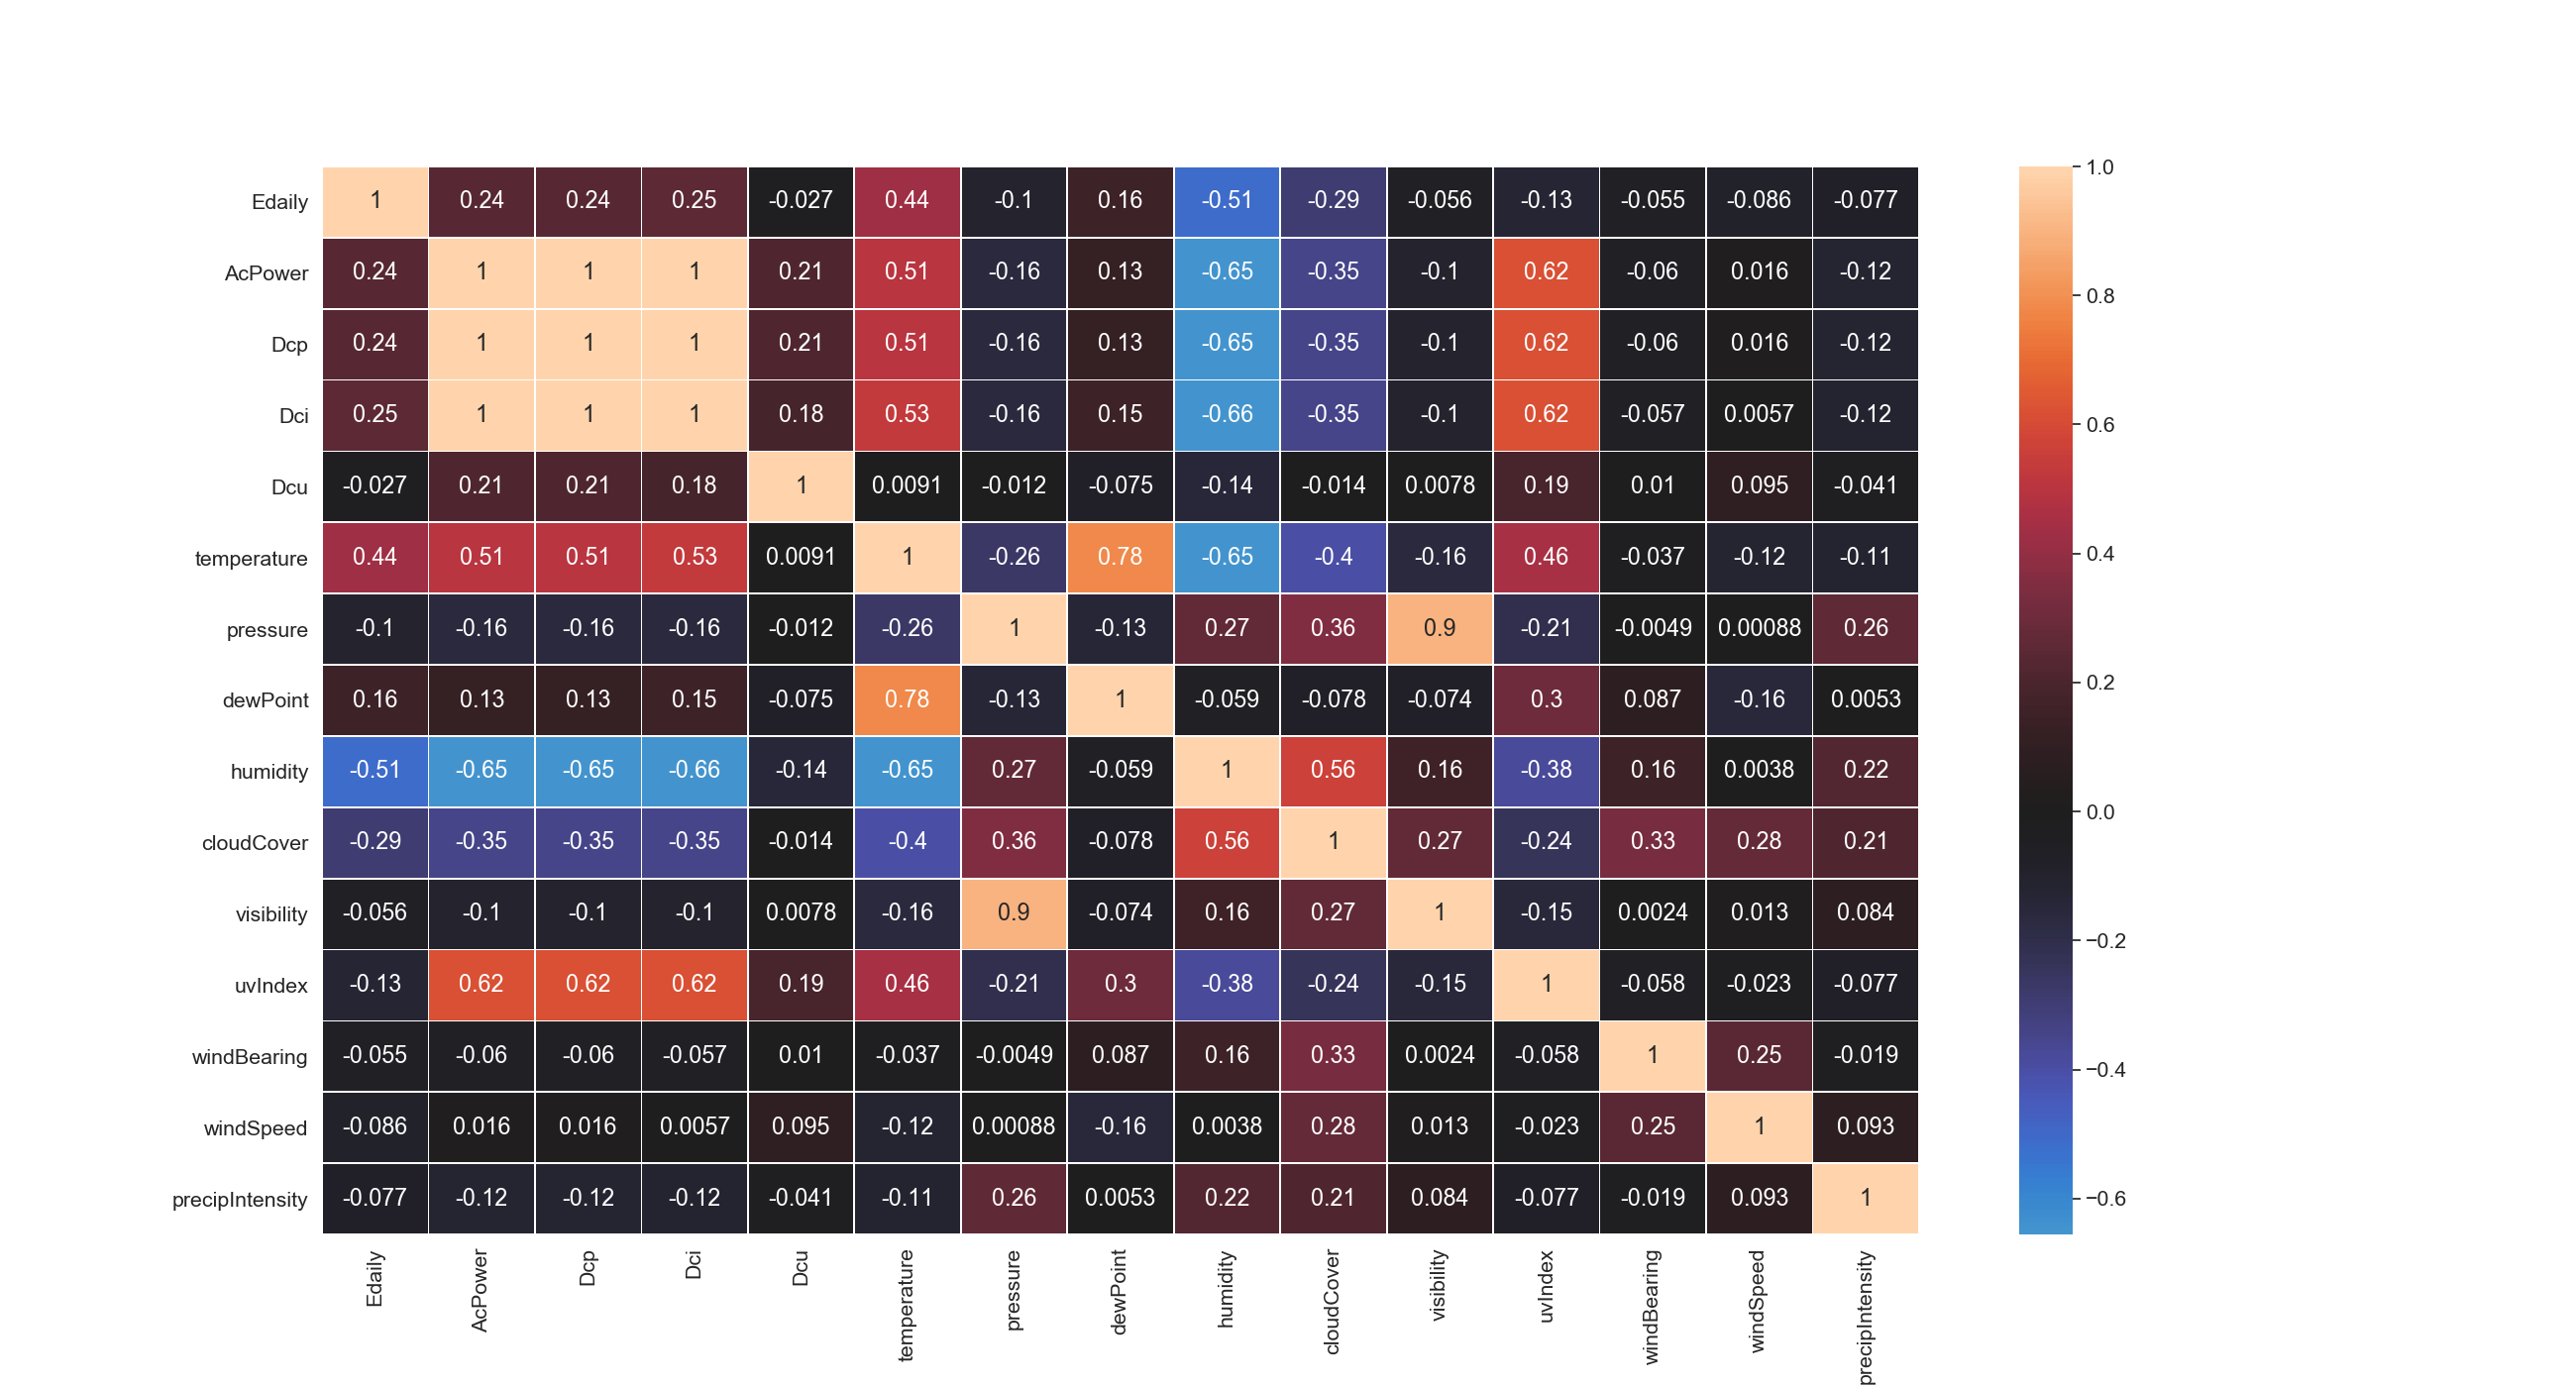
\includegraphics[height=0.8\textheight,trim={3cm 0 2cm 4cm},clip]{images/Heatmap.png}
\end{figure}
\end{frame}

\begin{frame}
\frametitle{Korrelation}
\begin{columns}[t]
	\column{.5\textwidth}
		\begin{figure}
			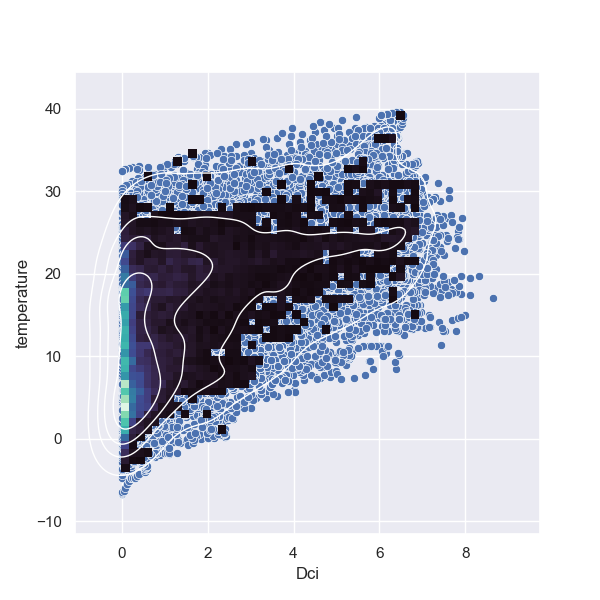
\includegraphics[width=\textwidth]{images/Dci_temperature.png}
		\end{figure}
	\column{.5\textwidth}
		\begin{figure}
			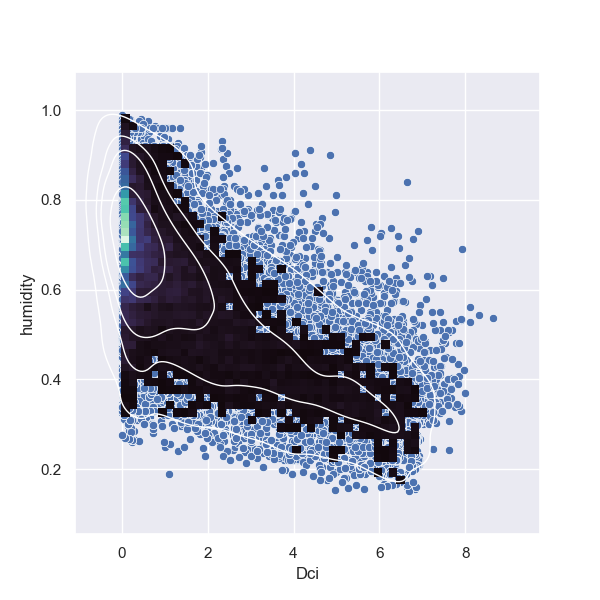
\includegraphics[width=\textwidth]{images/Dci_humidity.png}
		\end{figure}
\end{columns}
\end{frame}

\begin{frame}
\frametitle{Feature Vektor}
\begin{itemize}
	\item Dci: Gleichstrom (\si{\milli\ampere})
	\item Dcu: Gleichspannung (\si{\milli\volt})
	\item temperature: Lufttemperatur (\si{\celsius} )
	\item uvIndex: UV Index
	\item humidity: relative Luftfeuchtigkeit (0 bis 1)
	\item cloudCover: relative Wolkenbedeckung (0 bis 1)
	\item fracMinuteOfDay: Minute relativ zum ganzen Tag
	\item fracDayOfYear: Tag relativ zu ganzen Jahr
\end{itemize}
\end{frame}

\subsection{Klassifikation}

\begin{frame}
\frametitle{Klassifikation}
\begin{itemize}
	\item bekannt für einzelne Anlagen
	\begin{itemize}
		\item Diodenfehler: Gruibingen (ID 622592)
		\item Schatten: Banane 1 (ID 425987)\newline
	\end{itemize}
	\item Zuordnung anhand von String ID\newline
	\item Dataframe-Spalte \glq{}defect\grq (True/False)
\end{itemize}
\end{frame}

\subsection{Hauptkomponentenanalyse}
\begin{frame}
\frametitle{Hauptkomponentenanalyse}
Betrachtete Daten:
\begin{itemize}
	\item Diodenfehler: Grubingen (Hermann-Kirchheim)
	\item Anlage mit Schatten : Banana 1 (Globus-Erfurt-Mittelhausen)
	\item Zeitraum zwischen Januar 2019 und Juli 2019
	\item Fehlerhafte Strings extrahiert und binär klassifiziert
	\begin{itemize}
		\item Defekt und Okay
	\end{itemize}
	\item Merkmale
	\begin{itemize}
		\item Dci, Dcu, Temperatur, uvIndex, Luftfeucht, Bewölkung, relative Minute, relativer Tag
	\end{itemize}
\end{itemize}
\end{frame}

\begin{frame}
\frametitle{Hauptkomponentenanalyse}
\begin{itemize}
	\item Engl. Principal Components Analysis
	\item Reduzierung der Anzahl von statistischen Variablen
	\item Durchführung einer Hauptachsentransformation
	\item[$\rightarrow$] Reduzierung der Dimensionalität (z.B. zu 3D)
\end{itemize}
\end{frame}

\begin{frame}
\frametitle{Hauptkomponentenanalyse}
Durchführung:
\begin{itemize}
	\item Spaltenweise Subtraktion der jeweiligen Mittelwerte
	\item Bestimmung der Kovarianzmatrix
	\item Bestimmung der Eigenwerte und –vektoren
	\item Sortierung der Eigenvektoren absteigend nach deren Eigenwerten
	\item Auswahl einer Untermenge der Eigenvektoren
\end{itemize}
\end{frame}

\begin{frame}
\frametitle{Hauptkomponentenanalyse}
\begin{columns}[c]
	\column{.5\textwidth}
	im 2D-Raum
	\begin{itemize}
		\item Bestimmung Mittelwert
		\item Gerade durch Mittelwert, minimaler Summe der Orthogonalabstände
		\item Projektion der Datenpunkte auf diese Gerade
	\end{itemize}
	
	Bewertung
	\begin{itemize}
		\item Varianz der Projektion
		\item Je größer desto aussagekräftiger
	\end{itemize}
	
	\column{.5\textwidth}
	\begin{figure}
		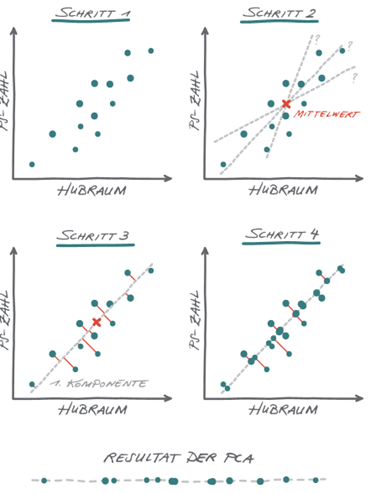
\includegraphics[width=\textwidth]{images/Hauptkomponentenanalyse.png}
	\end{figure}
\end{columns}
\end{frame}

\begin{frame}
\frametitle{HKA Schatten}
\begin{figure}
	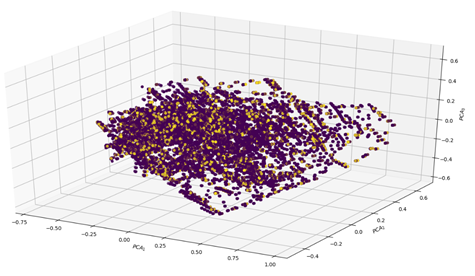
\includegraphics[width=0.47\textwidth]{images/Banane_1.png}
	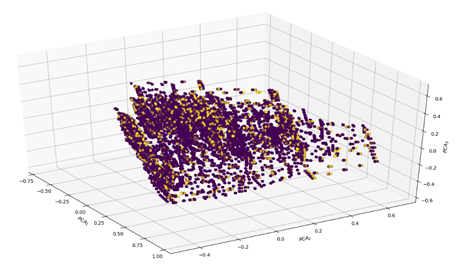
\includegraphics[width=0.47\textwidth]{images/Banane_2.png}
\end{figure}

PCA mit Reduzierung auf die drei Komponenten mit der höchsten Varianz: [0.521  0.204 0.126 ] 

\end{frame}

\begin{frame}
\frametitle{HKA Diodenfehler}
\begin{figure}
	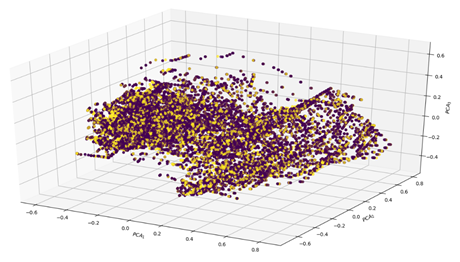
\includegraphics[width=0.47\textwidth]{images/Grubingen_1.png}
	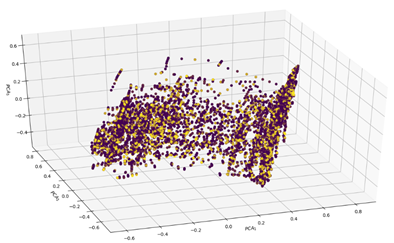
\includegraphics[width=0.47\textwidth]{images/Grubingen_2.png}
\end{figure}

PCA mit Reduzierung auf die drei Komponenten mit der höchsten Varianz: [0.525  0.226 0.139 ]
\end{frame}

\begin{frame}
\frametitle{Hauptkomponentenanalyse}
\begin{itemize}
	\item An beiden Standorten:
	\begin{itemize}
		\item Keine einfache Separation der Daten über PCA möglich
	\end{itemize}
	
	\item Interne Streuung der Merkmale größer als zwischen den Gruppen
	\begin{itemize}
		\item Interne Streuung der Merkmale größer als zwischen den Gruppen
		\item Defekte und korrekt arbeitende String vermutlich nicht linear separierbar
		\item Vermutlich komplexes neuronales Netz nötig
	\end{itemize}
\end{itemize}
\end{frame}

%------------------------------------------------
\section[ML-Experimente]{Machine-Learning-Experimente}
%------------------------------------------------

\subsection{Machine Learning Klassifikation}
\begin{frame}
\frametitle{Supervised Machine Learning-Modelle}
\begin{itemize}
	\item Mustererkennung durch supervised learning-Modelle\newline
	\item Alternative zu neuronalen Netzen
	\item Verzicht auf Komplexität
		\begin{itemize}
		\item Lange/Längere Einlernphase
		\item Optimierungen über Anzahl Layer und Neuronen entfallen
	\end{itemize}
\end{itemize}
\end{frame}

\begin{frame}
\frametitle{Modellevaluation}
\begin{figure}
	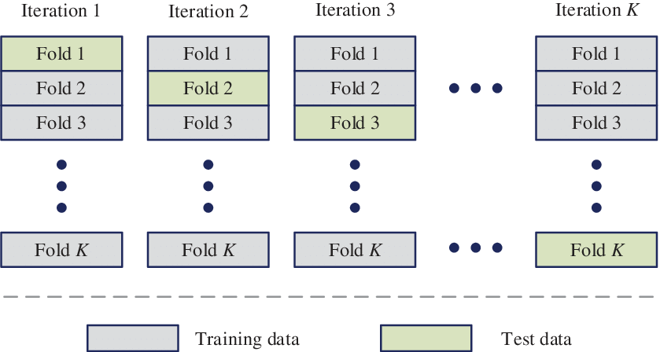
\includegraphics[width=\textwidth]{images/Modelle/k_fold_Cross_Validation.png}
\end{figure}
\end{frame}

\begin{frame}
\frametitle{SVM-Datensatz 1-Alle feature}
\begin{figure}
	\includegraphics[width=5cm,clip]{images/Alle feature/SVM_cross_val_1.png}
	\includegraphics[width=5cm,clip]{images/Alle feature/SVM_conf_1.png}
\end{figure}
\end{frame}

\begin{frame}
\frametitle{SVM-Datensatz 2-Alle feature}
\begin{figure}
	\includegraphics[width=5cm,clip]{images/Alle feature/SVM_cross_val_2.png}
	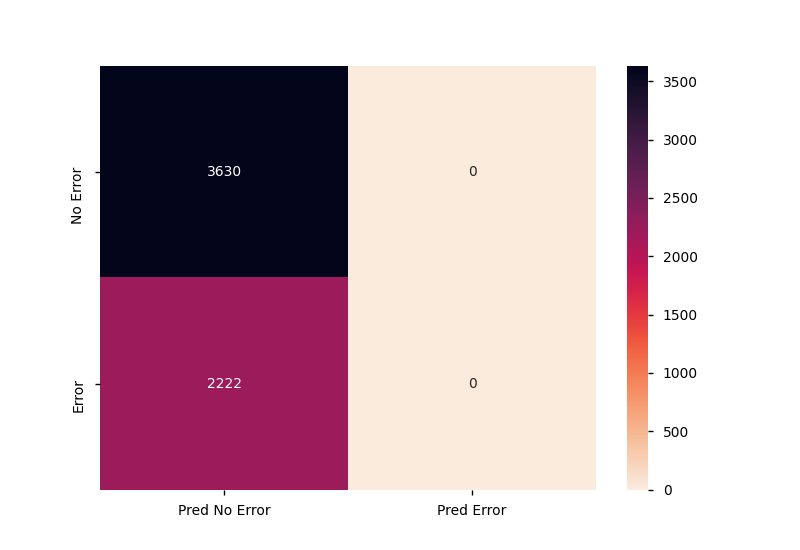
\includegraphics[width=5cm,clip]{images/Alle feature/SVM_conf_2.png}
\end{figure}
\end{frame}

\begin{frame}
\frametitle{SVM-Datensatz 3-Alle feature}
\begin{figure}
	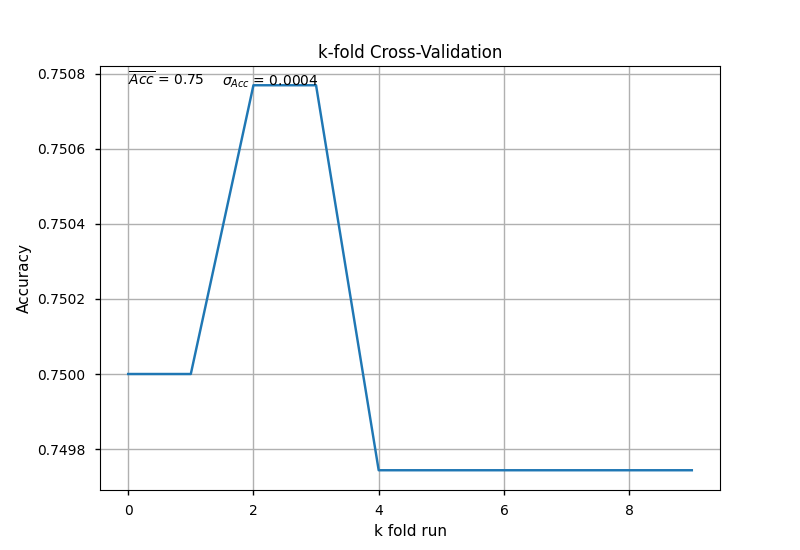
\includegraphics[width=5cm,clip]{images/Alle feature/SVM_cross_val_3.png}
	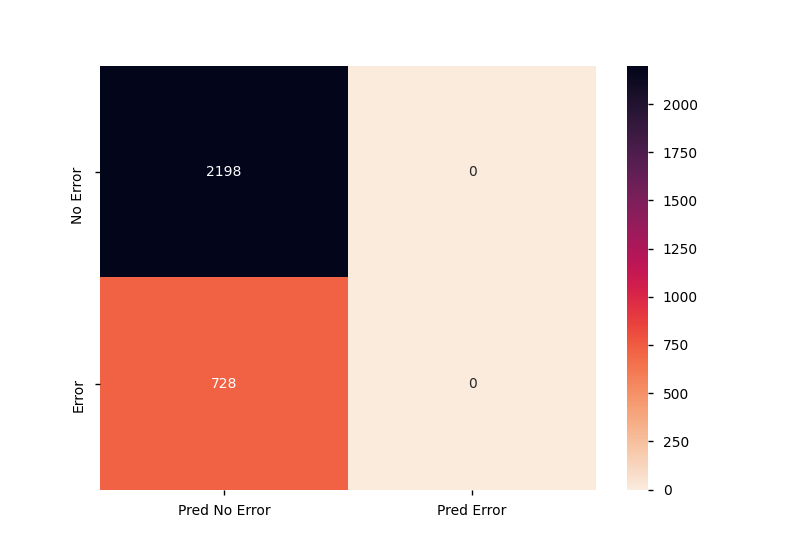
\includegraphics[width=5cm,clip]{images/Alle feature/SVM_conf_3.png}
\end{figure}
\end{frame}

\begin{frame}
\frametitle{KNN-Datensatz 1-Alle feature}
\begin{figure}
	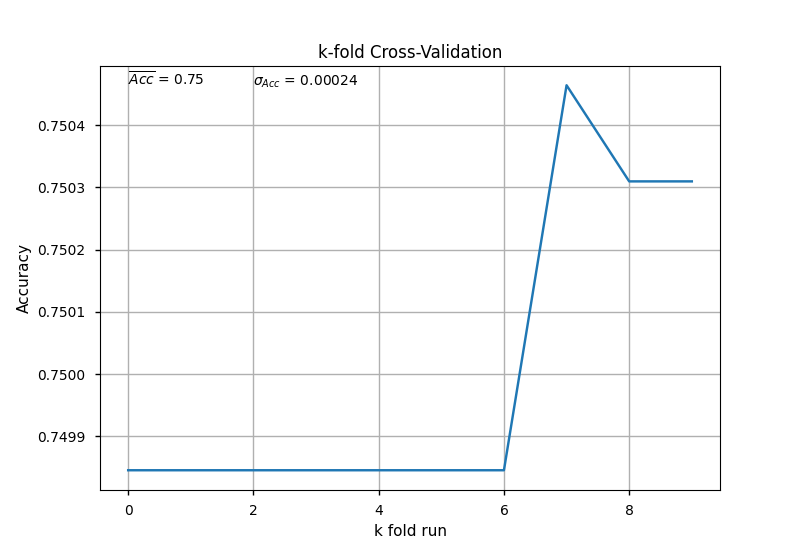
\includegraphics[width=5cm,clip]{images/Alle feature/KNN_cross_1.png}
	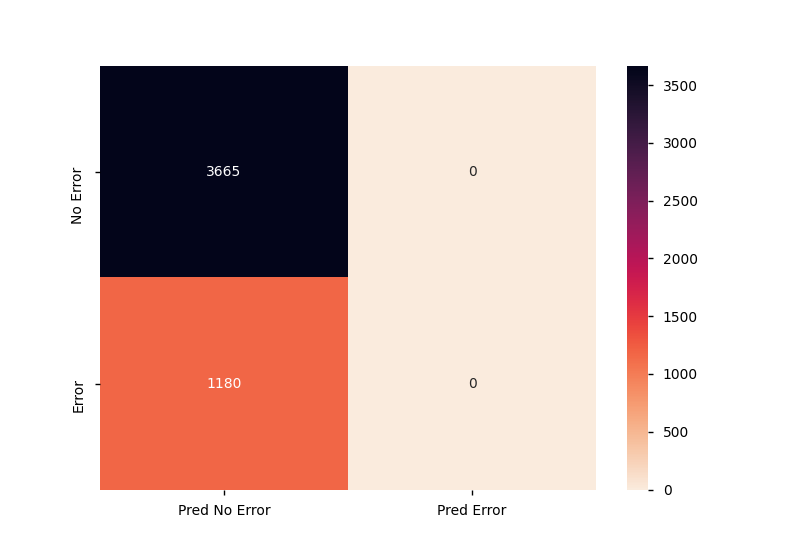
\includegraphics[width=5cm,clip]{images/Alle feature/KNN_conf_1.png}
\end{figure}
\end{frame}

\begin{frame}
\frametitle{KNN-Datensatz 2-Alle feature}
\begin{figure}
	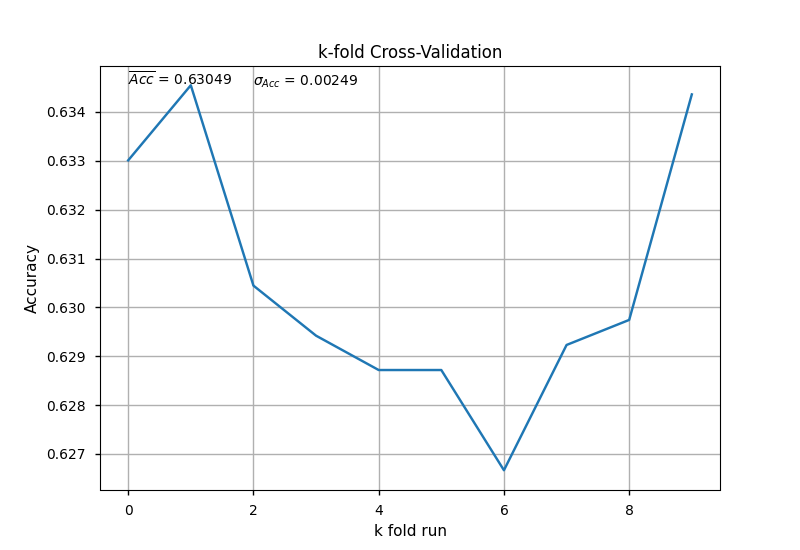
\includegraphics[width=5cm,clip]{images/Alle feature/KNN_cross_val_2.png}
	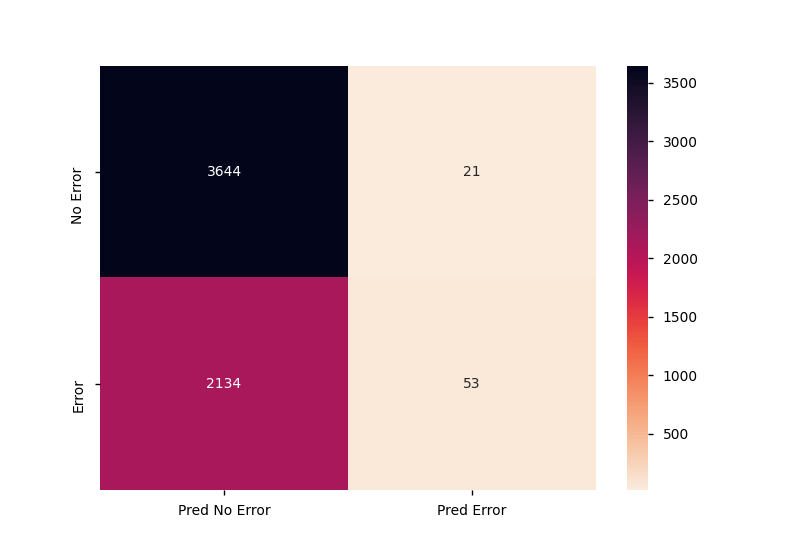
\includegraphics[width=5cm,clip]{images/Alle feature/KNN_conf_2.png}
\end{figure}
\end{frame}

\begin{frame}
\frametitle{KNN-Datensatz 3-Alle feature}
\begin{figure}
	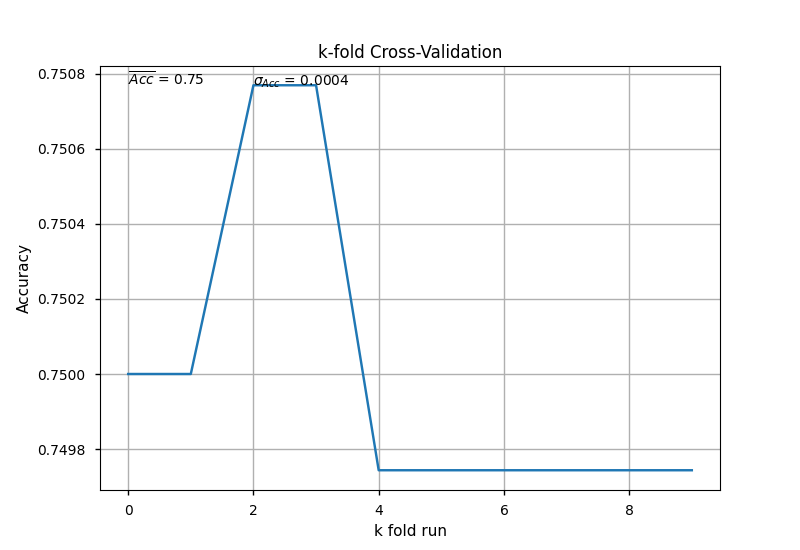
\includegraphics[width=5cm,clip]{images/Alle feature/KNN_cross_val_3.png}
	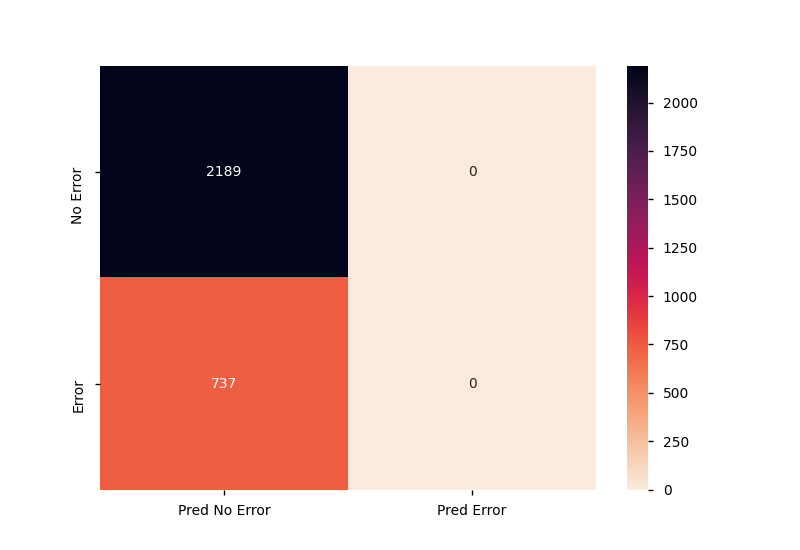
\includegraphics[width=5cm,clip]{images/Alle feature/KNN_conf_3.png}
\end{figure}
\end{frame}

\begin{frame}
\frametitle{Potnentielles Problem}
\begin{itemize}
	\item Daten anscheinend kaum/gar nicht separierbar?
	\item Möglichkeit: Feature Vector zu komplex?
	\item Weitere Feature-Reduktion durch RFE
\end{itemize}
\end{frame}

\begin{frame}
\frametitle{RFE}
\begin{figure}
	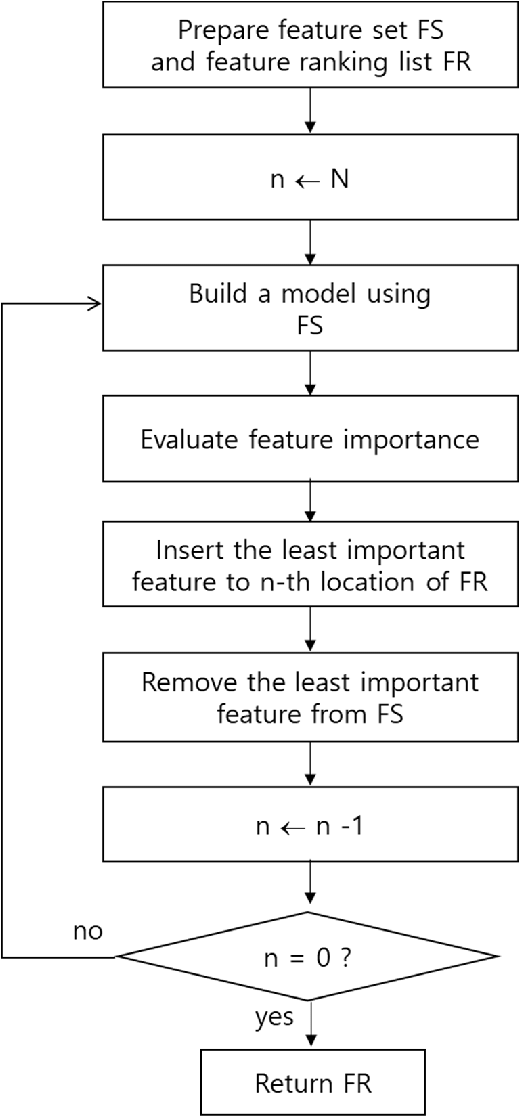
\includegraphics[width=3cm]{images/Modelle/RFE-Ablauf.png}
\end{figure}
\end{frame}

\begin{frame}
\frametitle{SVM-Datensatz 1-Reduzierte feature}
\begin{figure}
	\includegraphics[width=5cm,clip]{images/Reduzierte feature/SVM_cross_val_1.png}
	\includegraphics[width=5cm,clip]{images/Reduzierte feature/SVM_conf_1.png}
\end{figure}
\end{frame}

\begin{frame}
\frametitle{SVM-Datensatz 2-Reduzierte feature}
\begin{figure}
	\includegraphics[width=5cm,clip]{images/Reduzierte feature/SVM_cross_val_2.png}
	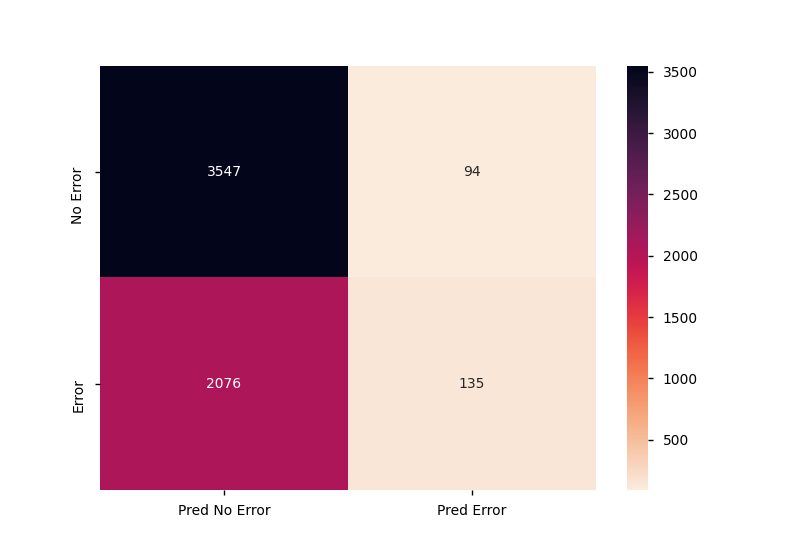
\includegraphics[width=5cm,clip]{images/Reduzierte feature/SVM_confl_2.png}
\end{figure}
\end{frame}

\begin{frame}
\frametitle{SVM-Datensatz 3-Reduzierte feature}
\begin{figure}
	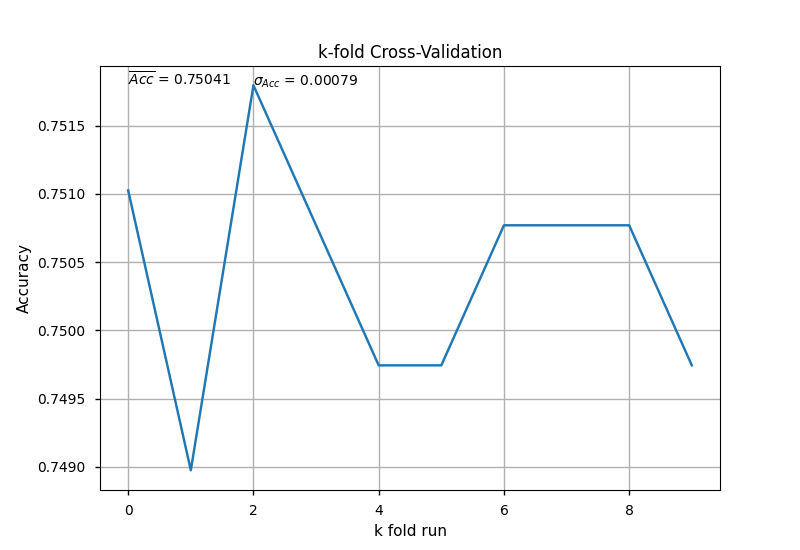
\includegraphics[width=5cm,clip]{images/Reduzierte feature/SVM_cross_val_3.png}
	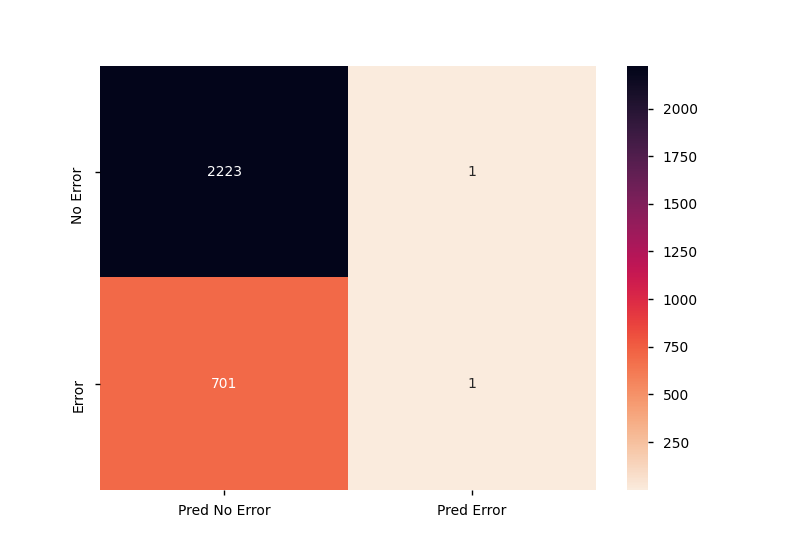
\includegraphics[width=5cm,clip]{images/Reduzierte feature/SVM_confl_3.png}
\end{figure}
\end{frame}

\begin{frame}
\frametitle{KNN-Datensatz 1-Reduzierte feature}
\begin{figure}
	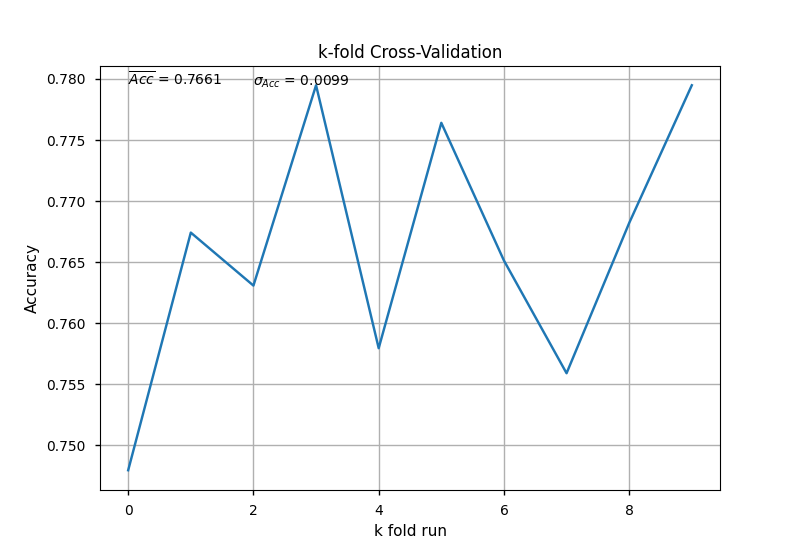
\includegraphics[width=5cm,clip]{images/Reduzierte feature/KNN_cross_val_1.png}
	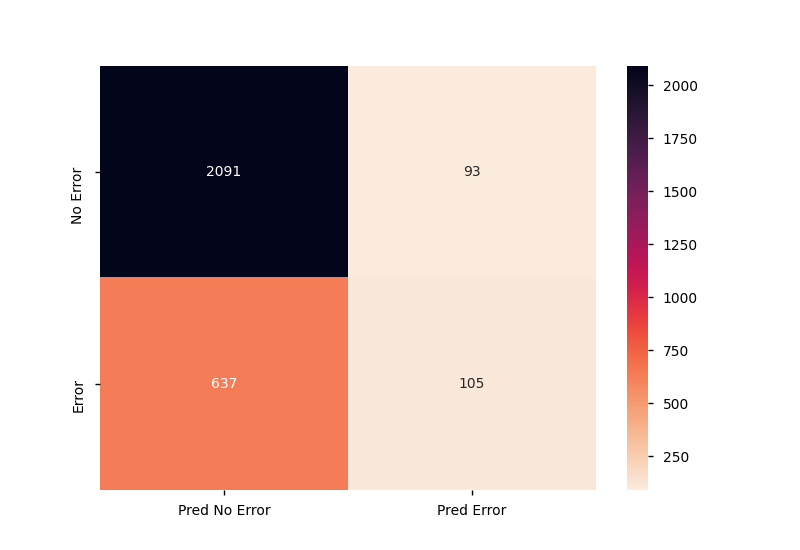
\includegraphics[width=5cm,clip]{images/Reduzierte feature/KNN_confl_1.png}
\end{figure}
\end{frame}

\begin{frame}
\frametitle{KNN-Datensatz 2-Reduzierte feature}
\begin{figure}
	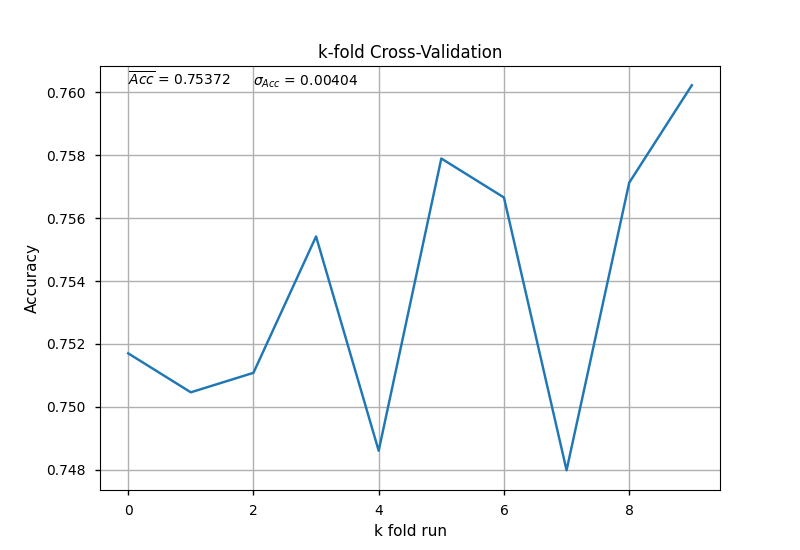
\includegraphics[width=5cm,clip]{images/Reduzierte feature/KNN_cross_val_2.png}
	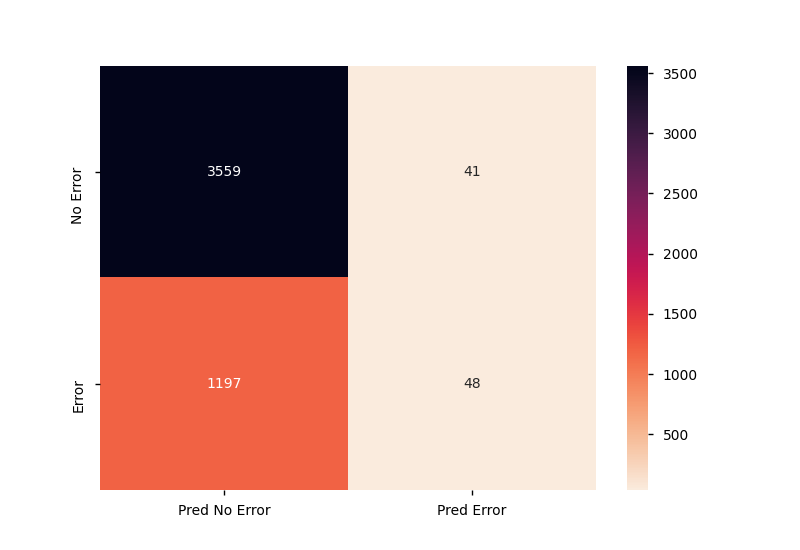
\includegraphics[width=5cm,clip]{images/Reduzierte feature/KNN_conf_2.png}
\end{figure}
\end{frame}

\begin{frame}
\frametitle{KNN-Datensatz 3-Reduzierte feature}
\begin{figure}
	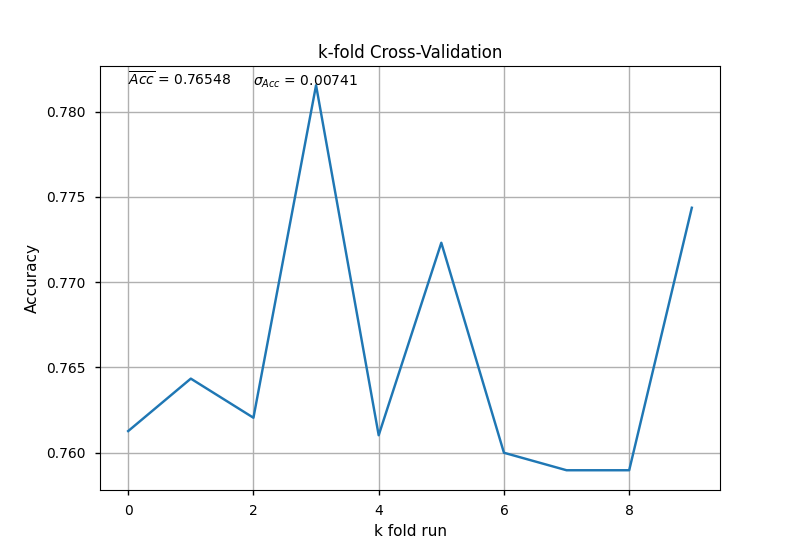
\includegraphics[width=5cm,clip]{images/Reduzierte feature/KNN_cross_val_3.png}
	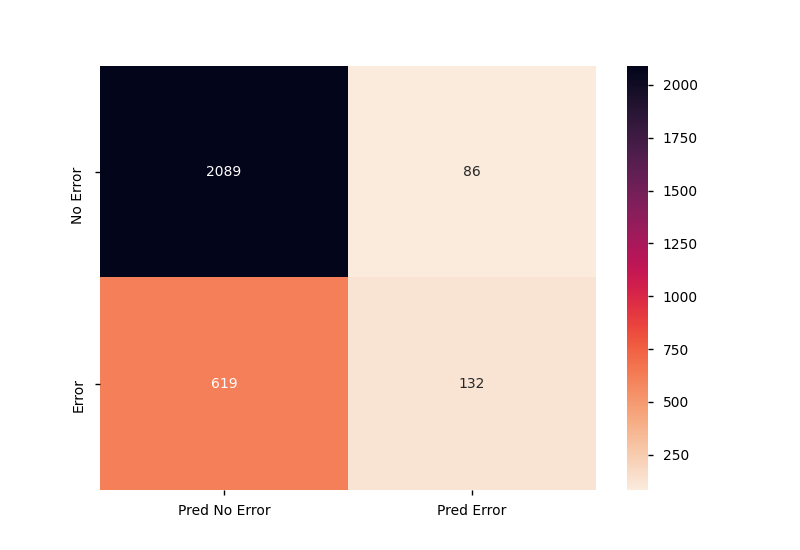
\includegraphics[width=5cm,clip]{images/Reduzierte feature/KNN_confl_3.png}
\end{figure}
\end{frame}

\begin{frame}
\frametitle{Schlussfolgerung für weiteren Nutzen}
\begin{itemize}
	\item Nach wie vor schlechte Ergebnisse
		\begin{itemize}
		\item Stets Abhängigkeit von relativen Häufigkeiten der Ergebnisse
		\item Daten können auf dem Wege nicht getrennt werden\newline
	\end{itemize}
	\item Methodik wird verworfen\newline
	\item Keine Gewinne aus statischen Daten?
\end{itemize}
\end{frame}


\subsection{Einfaches neuronale Netz}
\begin{frame}
\frametitle{Einfaches neuronales Netz}
\begin{itemize}
	\item Modell: keras.models.Sequential (einfache Schichtung)
	\begin{itemize}
		\item Loss: zu minimierende Größe
		\item Optimizer: Optimierungsstrategie\newline
	\end{itemize}

	
	\item Schichten
	\begin{itemize}
		\item keras.layers.core.Dense: regular densely-connected NN layer
		\begin{itemize}
			\item Units: Anzahl Neuronen
			\item Activation: Aktivierungsfunktion
		\end{itemize}
		\item keras.layers.core.Dropout: verringert Overfitting\newline
	\end{itemize}
	
	\item Daten
	\begin{itemize}
		\item Anlage: Banane 1
		\item Gruppe: südwestl-Eingänge
		\item Sample: 10000 Werte (Anteil Klassen: 50/50)
		\item Train-Test-Split: 70/30
	\end{itemize}
\end{itemize}
\end{frame}

\begin{frame}
\frametitle{NN Training}
\begin{figure}
	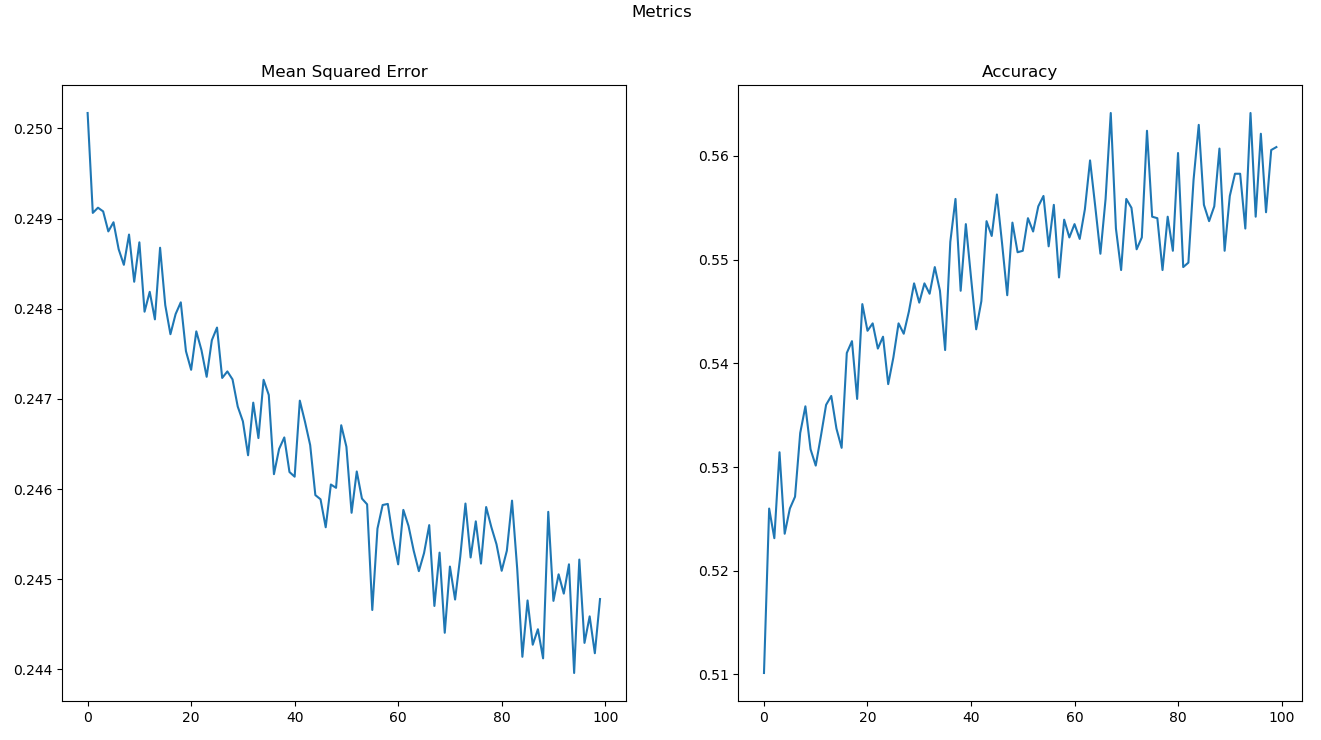
\includegraphics[width=\textwidth]{images/NN-Training_Baseline.png}
\end{figure}
\end{frame}

\begin{frame}
\frametitle{NN Varianten}
\begin{tabular}{c|c|c|c|c}
	Loss & Optimizer & Units & Activation & Accuracy\\
	\hline
	MSE & adam    & [8,16,5,1]    & relu    & 0.5337\\
	MSE & RMSprop & [8,16,5,1]    & relu    & 0.5423\\
	MSE & adam    & [8,16,5,1]    & sigmoid & 0.5133\\
	MSE & adam    & [8,16,8,4,2,1]& relu    & 0.5503\\
\end{tabular}
\end{frame}

\subsection{Rekurrentes neuronales Netz}
\begin{frame}
\frametitle{Rekurrentes neuronales Netz}
\begin{itemize}
	\item Modell: keras.models.Sequential\newline
	
	\item Schichten
	\begin{itemize}
		\item keras.layers.CuDNNLSTM
		\begin{itemize}
			\item Long Short-Term Memory (LSTM) Schicht
			\item läuft auf GPU
		\end{itemize}
		\item keras.layers.core.Dropout\newline
	\end{itemize}
	
	\item Daten
	\begin{itemize}
		\item Anlage: Banane 1
		\item Gruppe: südwestl-Eingänge
	\end{itemize}
\end{itemize}
\end{frame}

\begin{frame}
\frametitle{LSTM Training}
\begin{figure}
	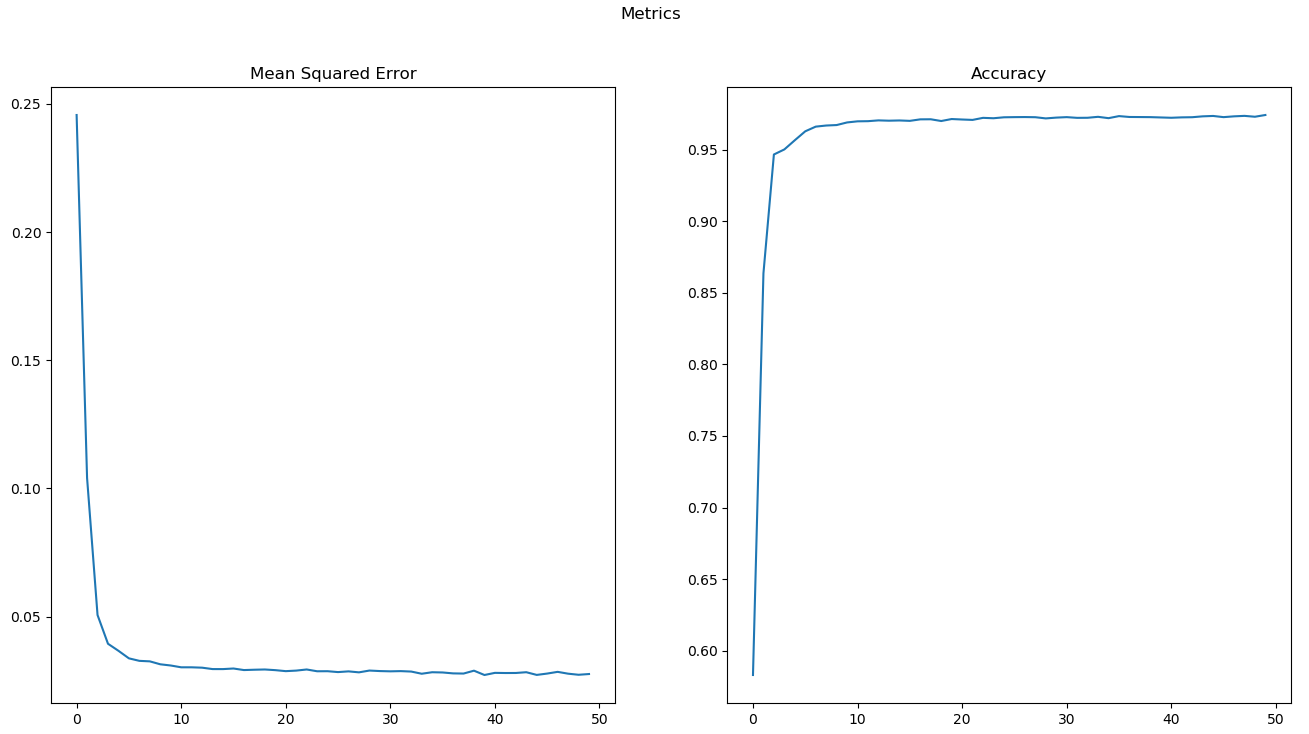
\includegraphics[width=\textwidth]{images/LSTM-Training.png}
\end{figure}
\end{frame}

\begin{frame}
\frametitle{Weitere Experimente}
Beschränkung der Training-/Testdaten auf Mittagszeit (12:00 - 15:00)\newline
\begin{itemize}
	\item NN: keine Verbesserung (Accuracy $0.534 \rightarrow 0.532$)
	\item LSTM: keine Verbesserung (Accuracy $0.974 \rightarrow 0.970$)
\end{itemize}
\end{frame}

%------------------------------------------------
\section{Ergebnisse}
%------------------------------------------------

\begin{frame}
\frametitle{Ergebnisse}
Lassen sich Modulfehler von Photovoltaikanlagen mit Hilfe von maschinellem Lernen anhand von Leistungs- und Wetterdaten zuverlässig erkennen und klassifizieren?\newline
\begin{itemize}
	\item SVM:
	\begin{itemize}
		\item keine ausreichende Trennung
		\item abhängig von rel. Häufigkeit der Klassen
	\end{itemize}
	\item neuronales Netz
	\begin{itemize}
		\item inkonsistente Lernrate
		\item Accuracy: 0.55 (sample), 0.713 (alle Daten)
		\item abhängig von rel. Häufigkeit der Klassen?
	\end{itemize}
	\item LSTM Netz (50 Epochen)
	\begin{itemize}
		\item Schatten: Accuracy $\approx 0.974$
		\item Diodenfehler: Accuracy $\approx 0.954$
	\end{itemize}
\end{itemize}
\end{frame}

\begin{frame}
\frametitle{Ergebnisse}
Lässt sich die Erkennung von Modulfehlern durch das Einbeziehen simulierter Daten verbessern?\newline
\begin{itemize}
	\item aus Zeitgründen nicht mehr bearbeitet
	\item simulierte Daten nicht kompatible mit Messdaten (keine Wetterinformationen)
\end{itemize}
\end{frame}

%------------------------------------------------
\section{Fazit}
%------------------------------------------------

\begin{frame}
\frametitle{Fazit}
\begin{itemize}
	\item SVM und reguläre NN zu klein für Problemstellung ($<1500$ Parameter)\newline
	\item LSTM Netz ($\sim 10000$ Parameter) liefert gute Ergebnisse\newline
	\item Schatten/Diodenfehler separat behandelt (verschiedene Anlagen)
\end{itemize}
\end{frame}

% Normale NN zu klein (< 1500 Parameter)
% LSTM Netze lieren gut Ergebnisse (~10000 Parameter)
% Erkennen möglich
% Klassifizieren?

%----------------------------------------------------------------------------------------

\end{document} 
